\documentclass[cic,tc]{iiufrgs}
\usepackage[utf8]{inputenc}   % pacote para acentuação
\usepackage{graphicx}         % pacote para importar figuras
\usepackage{times}            % pacote para usar fonte Adobe Times
\usepackage{algpseudocode}
\usepackage{url}
\usepackage{amsmath}
% \usepackage{palatino}
% \usepackage{mathptmx}       % p/ usar fonte Adobe Times nas fórmulas
\usepackage[alf,abnt-emphasize=bf]{abntex2cite}	% pacote para usar citações abnt

%
% Informações gerais
%
\title{Estudo e otimização dos softwares de bioinformática do Hospital de
Clínicas de Porto Alegre}

\author{Farah}{Alef}

% orientador e co-orientador são opcionais (não diga isso pra eles :))
\advisor[Prof.~Dr.]{Geyer}{Claudio Fernando Resin}
\coadvisor[Prof.~Dr.]{Anjos}{Julio Cesar Santos}

% a data deve ser a da defesa; se nao especificada, são gerados
% mes e ano correntes
\date{novembro}{2021}

% o local de realização do trabalho pode ser especificado (ex. para TCs)
% com o comando \location:
\location{Porto Alegre}{RS}

% itens individuais da nominata podem ser redefinidos com os comandos
%
% palavras-chave
% iniciar todas com letras minúsculas, exceto no caso de abreviaturas
%
\keyword{bioinformática}
\keyword{paralelismo}
\keyword{codeml}
\keyword{PAML}
\keyword{SAMtools}
%\keyword{}

%\settowidth{\seclen}{1.10~}

\begin{document}

% folha de rosto
% às vezes é necessário redefinir algum comando logo antes de produzir
% a folha de rosto:
% \renewcommand{\coordname}{Coordenadora do Curso}
\maketitle

% dedicatoria
% \clearpage
% \begin{flushright}
%     \mbox{}\vfill
%     {\sffamily\itshape
%       ``If I have seen farther than others,\\
%       it is because I stood on the shoulders of giants.''\\}
%     --- \textsc{Sir~Isaac Newton}
% \end{flushright}

% agradecimentos
%\chapter*{Agradecimentos}
%Agradeço ao \LaTeX\ por não ter vírus de macro\ldots

% resumo na língua do documento
\begin{abstract}
  Neste trabalho foi realizado um estudo e otimização dos problemas de
  desempenho presentes em alguns dos softwares de bioinformática utilizados
  pelo grupo de pesquisa em genética do Hospital de Clínicas de Porto Alegre
  (HCPA), empregando para isso técnicas de processamento paralelo. O trabalho
  focou no software de análise filogenética codeml, do pacote PAML, amplamente
  utilizado na literatura, e no software SAMtools, usado para chamada de
  variantes, igualmente popular. Foi desenvolvida uma ferramenta de
  paralelização de \textit{jobs} do SAMtools, reduzido de vários dias para
  poucas horas o tempo de análise do grupo de pesquisa, enquanto que no caso do
  codeml foi realizado uma análise de desempenho de alternativas encontradas em
  revisão bibliográfica, fornecendo aos pesquisadores uma ferramenta que reduz
  em mais da metade o tempo de execução em relação ao codeml original.
  \end{abstract}

% resumo na outra língua
% como parametros devem ser passados o titulo e as palavras-chave
% na outra língua, separadas por vírgulas
\begin{englishabstract}{Study and optimization of the bioinformatics software used by Hospital de Clínicas de Porto Alegre}{Bioinformatics, parallelism, codeml, PAML, SAMtools} In this paper we studied and optimized the performance bottlenecks found in some of the bioinformatics software used by the genetics research group from Hospital de Clínicas de Porto Alegre (HCPA), employing parallel programming techniques to achieve these goals. The focus of our work was in the phylogenetic analysis software called codeml, from the PAML package, which is widely used in the literature, as well on the SAMtools software, used for variant calling, also popular. We developed a tool for the parallel execution of SAMtools jobs, reducing total execution time for the group's input from various days to a few hours, while in the case of codeml we analyzed the performance of solutions found in a bibliography review, supplying the researches with a tool whose execution time is half that of codeml.
\end{englishabstract}

% lista de figuras
\listoffigures

% lista de tabelas
\listoftables

% lista de abreviaturas e siglas
% o parametro deve ser a abreviatura mais longa
\begin{listofabbrv}{POSIX}
    \item[POSIX] \textit{Portable Operating System Interface}
    \item[HCPA] Hospital de Clínicas de Porto Alegre
    \item[GATK] \textit{Genome Analysis Toolkit}
    \item[PAML] \textit{Phylogenetic Analysis By Maximum Likelihood}
    \item[NCBI] \textit{National Center for Biotechnology}
    \item[BFGS] Broyden–Fletcher–Goldfarb–Shanno
    \item[CPU] \textit{Central Processing Unit}
    \item[GPU] \textit{Graphics Processing Unit}
    \item[API] \textit{Application Programming Interface}
    \item[DNA] Ácido desoxirribonucleico
    \item[RNA] Ácido ribonucleico
    \item[RAM] \textit{Random access memory}
    \item[ARC] \textit{Advanced Resource Connector}
    \item[PBS] \textit{Population Branch Statistic}
    \item[GRC] \textit{Genome Reference Consortium}
    \item[IPC] \textit{Inter process communication}
    \item[GHz] Giga hertz
    \item[GB] Giga byte
    \item[TB] Tera byte
    \item[IO] \textit{Input output}
\end{listofabbrv}

% idem para a lista de símbolos
\begin{listofsymbols}{$F_{ST}$}
    \item[$\omega$] Taxa de substituição
    \item[$dN$] Substituições não-sinônimas
    \item[$dS$] Substituições sinônimas
    \item[$F_{ST}$] Índice de fixação
    \item[$\frac{\partial f}{\partial x_i}$] Derivada parcial de $f$ com respeito a $x_i$
\end{listofsymbols}

% sumario
\tableofcontents

% aqui comeca o texto propriamente dito

% introducao
\chapter{Introdução}

Neste trabalho foi realizado um estudo e otimização dos problemas de desempenho
presentes em alguns dos softwares de bioinformática utilizados pelo grupo de
pesquisa em genética do Hospital de Clínicas de Porto Alegre (HCPA), empregando
para isso técnicas de processamento paralelo e distribuído sempre que viável.

Nomeadamente foram estudados os softwares codeml, do pacote
PAML,\cite{yang2007paml} amplamente utilizado na literatura para análise
filogenética;\cite{maldonado2016lmap} o pacote ANGSD, utilizado para comparação
de sequências genéticas de diferentes populações de uma
espécie;\cite{korneliussen2014angsd} e o pacote SAMtools, amplamente utilizado
na literatura para manipulação de arquivos de sequências genéticas
alinhadas e chamada de variantes,\cite{danecek2021twelve} e usado pelo grupo
como uma alternativa ao software ANGSD.

Cada um desses softwares apresentava problemas de desempenho diferentes dentro
do pipeline de análise genética do grupo de pesquisa. Nomeadamente, o PAML e o
SAMtools apresentavam tempos de execução proibitivamente elevados, enquanto que
o ANGSD apresentava uso de memória proibitivamente alto. No caso dos softwares
PAML e ANGSD foram realizadas análises de desempenho dos softwares originais
bem como de alternativas encontradas através de um estudo da literatura,
enquanto que no caso do pacote SAMtools foi desenvolvida uma ferramenta para
execução de \textit{jobs} paralelos para ambientes multiprocessados, bem como
uma interface gráfica para uso desse ferramental.

A identificação de softwares alternativos ao PAML através do estudo e análise
supracitados resultaram na economia de mais da metade do tempo de execução para
os dados de entrada do grupo de pesquisa do HCPA, enquanto que a ferramenta
desenvolvida para paralelização de \textit{jobs} do SAMtools reduziu de dias
para horas o tempo da análise realizada pelo grupo com essa ferramenta,
permitindo que ela fosse utilizada como alternativa ao software ANGSD, cujos
problemas de desempenho foram mapeados através de um perfil de execução, mas
não foram atacados nesse trabalho, sendo a ferramenta de paralelização do
SAMtools a alternativa favorecida.
% TODO especificar o antes e depois exato do SAMtools

\section{Conceitos de bioinformática}

A fim de compreender o uso e funcionamento dos softwares que foram objeto de
estudo desse trabalho, convém elucidar alguns conceitos de bioinformática. Na
seção \ref{sec:filo} é apresentado o conceito de análise filogenética, objeto
de estudo dos usuários do pacote PAML, na seção \ref{sec:call} é exposto o
conceito de análise de variações genéticas de diferentes populações de uma
espécie através de um processo denominado chamada de variantes, para o qual os
pacotes ANGSD e SAMtools são empregados, e na seção \ref{sec:formats} são
brevemente expostos os formatos de arquivos utilizados para cada um desses
processos.

\subsection{Análise filogenética}
\label{sec:filo}

A análise filogenética, propósito do PAML, compreende o estudo da evolução de
um ou mais organismos e suas características. Nesta sessão são brevemente
apresentados alguns conceitos de análise filogenética relevantes ao
entendimento dos softwares utilizados e seu comportamento.

A informação genética presente no DNA dos seres vivos é utilizada no processo
de síntese proteica, onde os códons (tripla de nucleotídeos) presentes no RNA
mensageiro, gerado a partir do DNA, determinam a síntese de aminoácidos
específicos, componentes das proteínas, macromoléculas fundamentais à vida.

Existem quatro tipos de nucleotídeos no código genético, formados por adenina
(A), guanina (G), uracila (U), e citosina (C). Dessa forma, existem $4^3 = 64$
códons distintos, dos quais três são códons de terminação, que indicam o fim da
etapa de tradução na síntese proteica, enquanto os outros 61 códons traduzem
para um aminoácido específico.

Apenas 20 aminoácidos compõem as proteínas em seres vivos. Sendo assim, a
maioria dos aminoácidos é traduzido por mais de um códon. Em outras palavras, a
substituição de certos códons no DNA não produz alteração nos aminoácidos
gerados na síntese proteica.

As substituições que não geram alterações na síntese proteica são chamadas de
sinônimas ou silenciosas, enquanto as que modificam os aminoácidos gerados são
não sinônimas. Acredita-se que as substituições sinônimas sejam mais comuns e
não sofram tanta pressão seletiva. A taxa de substituições sinônimas e não
sinônimas $\omega = \frac{dN}{dS}$ é uma medida de seleção natural, conforme a
tabela abaixo.\cite{yang2002codon}

\begin{table}[h]
    \caption{Taxas de substituição}
    % OBS: não use \begin{center}, pois este aumenta o espaçamento entre a caption/legend e a tabela
    % Para figuras, a aparência é melhor com o espaçamento extra
    \centering
        \begin{tabular}{c|c}
          \hline
          \textit{Taxa}  &   \textit{Seleção} \\
          \hline
          \hline
          $\omega = 1$ & Seleção neutra \\
          $\omega < 1$ & Seleção negativa ou purificadora \\
          $\omega > 1$ & Seleção positiva \\
          \hline
        \end{tabular}
      \legend{Fonte: \cite{yang2002codon}}
    \label{tbl:ex1}
\end{table}

Em síntese, o propósito de softwares de análise filogenética como o pacote PAML
é detectar eventos de seleção positiva nas diferentes linhagens da árvore
filogenética de uma espécie. Para isso, softwares como o PAML utilizam modelos
estatísticos de máxima verossimilhança para comparar a hipótese de ocorrência
desses eventos contra a hipótese nula de seleção neutra ou
negativa.\cite{moretti2012gcodeml}

\subsection{Chamada de variantes}
\label{sec:call}

Um dos objetos de estudo da bioinformática é a compreensão dos genes envolvidos
em variações fenotípicas observadas entre diferentes populações de uma
espécie, em particular da espécie humana.\cite{jiang2019population} Para isso,
uma possibilidade é o estudo a nível molecular das variações genéticas entre
indivíduos de diferentes populações. A identificação dessas variações é
denominada ``chamada de variantes'' ou \textit{SNV calling}, o pacote SAMtools
providenciando ferramental para realização desse
processo.\cite{pirooznia2014validation} Existem diversos métodos para
identificação e análise dessas variações, um desses métodos sendo o
\textit{Population Branch Statistic} ou PBS,\cite{jiang2019population} para o
qual pode ser empregado o software ANGSD.

Uma métrica de diferença na estrutura genética entre duas populações de uma
espécie é o índice de fixação ou $F_{ST}$, baseado, em suma, na variança da
frequência alélica das duas populações. Genes com um $F_{ST}$ alto são
potenciais alvos de seleção natural.\cite{yi2010sequencing} Como o $F_{ST}$ é
uma métrica de comparação de pares, ele não é capaz de identificar a direção
das mudanças, nem pode ser utilizado como única métrica para identificar
eventos de seleção natural. O PBS consiste de um método estatístico que
utiliza comparações em pares do $F_{ST}$ entre três populações distintas para
quantificar as diferenças entre suas sequências genéticas. Genes com valor
PBS alto indicam seleção positiva.\cite{jiang2019population} Uma descrição
mais aprofundada do método foge ao escopo desse trabalho, e pode ser
encontrada em \cite{yi2010sequencing}.

Os pesquisadores do HCPA utilizam os pacotes ANGSD e SAMtools para realizar
a chamada de variantes visando entender variações fenotípicas entre populações
humanas, utilizando para isso o método PBS.

\subsection{Formatos de arquivos}
\label{sec:formats}

Fundamental ao entendimento de algumas otimizações realizadas nesse trabalho é
um conhecimento básico dos diferentes formatos de arquivo utilizados para
armazenamento de informação genética, no campo da bioinformática. Neste
trabalho foram trabalhados com arquivos nos formatos SAM, BAM, CRAM, BCF, VCF,
FASTA, e NWK, descritos brevemente nesta seção.

Os formatos SAM, BAM, e CRAM, representam sequências genéticas alinhadas a um
genoma de referência. O formato SAM traz uma representação em texto plano, o
BAM é seu equivalente binário, e o CRAM é uma versão binária com compressão.
Tais arquivos podem ser manipulados com a ferramenta samtools, do pacote
SAMtools.\cite{danecek2021twelve} Amostras de sequências genéticas de
indivíduos da espécie humana são fornecidos no formato CRAM pelo projeto 1000
Genomes, um esforço colaborativo internacional que visa sequenciar o genoma
humano e disponibilizar a informação publicamente.\cite{via20101000}

A chamada de variantes realiza comparações entre múltiplos arquivos nos
formatos supracitados, produzindo arquivos que representam as variantes
encontradas. Quando as informações de variantes são armazenadas em texto plano
diz-se do arquivo VCF, seu equivalente binário sendo o formato BCF, ambos
gerados e manipulados pela ferramenta bcftools, do pacote
SAMtools.\cite{danecek2021twelve}

Já o formato FASTA é utilizado para representar sequências
de nucleotídeos ou aminoácidos. Introduzido pela primeira vez em
\cite{fasta}, é hoje ubíquo no campo da
bioinformática.\cite{shen2016seqkit} Os genomas de referência aos quais as
demais sequências genéticas são alinhadas são fornecidos nesse formato, e o
pacote SAMtools providencia ferramental para manipulação desses arquivos. O
genoma de referência é publicado pelo órgão \textit{Genome Reference
Consortium} (GRC), e a publicação mais atual é nomeada GRCh38, de
2013.\cite{GUO201783} Além disso, o software PAML recebe arquivos nesse formato.

% TODO Convém entrar no mérito disso?
Convém mencionar que o projeto 1000 Genomes fornece ainda sequências alinhadas
ao genoma de referência anterior, GRCh37, no formato BAM, consideravelmente
maior que o CRAM. Esses arquivos, diferente dos mais recentes no formato CRAM e
alinhados ao GRCh38, encontram-se disponíveis em \textit{mirrors} como do
\textit{National Center for Biotechnology} (NCBI), providenciando maior largura
de banda.\cite{clarke20121000}

Por fim, para o software PAML, além de arquivos FASTA contendo as sequências
genéticas dos indivíduos da árvore filogenética, a árvore em si consiste de uma
das entradas do software. A árvore é fornecida no formato NWK ou Newick, um
formato texto plano com representação flexível, que basicamente separa os nodos
por vírgula e utiliza parênteses para distinguir nodos internos de folhas.
Originalmente introduzido na aplicação PHYLIP \cite{felsenstein1993phylip}, é
amplamente utilizado para representação de árvores filogenéticas.\cite{fredslund2006phy}

\chapter{Desenvolvimento}

\section{Pacote PAML}

O \textit{Phylogenetic Analysis by Maximum Likelihood} (PAML) é um pacote de
software com ferramentas para análise filogenética utilizando métodos
estatísticos de máxima verossimilhança.\cite{yang2007paml} Dentre
outras ferramentas disponíveis no pacote se destaca o codeml,
amplamente utilizado na literatura.\cite{maldonado2016lmap} Apesar de
estatisticamente robusto,\cite{maldonado2016lmap} o codeml possui
implementação ingênua de métodos numéricos computacionalmente
custosos.\cite{yang2020paml} Para o caso de uso do grupo de pesquisa em
genética do HCPA, o tempo de execução é de vários dias.

Neste trabalho foi realizada uma revisão bibliográfica a respeito do software
em questão e de alternativas a ele; foram realizadas análises de seu desempenho
através de perfis de execução, identificando as rotinas responsáveis pela maior
parte do tempo de execução; os gargalos de desempenho foram estudados através
de análise do código fonte e do manual da ferramenta, em seguida foi realizada
revisão bibliográfica a respeito dos métodos numéricos empregados, visando sua
otimização. Foram implementadas estratégias de paralelização de tais métodos e
realizadas novas análises de desempenho e de corretude do software
paralelizado. Por fim, foram realizadas análises de desempenho de softwares
alternativas encontrados no estudo da literatura.

\subsection{Trabalhos anteriores}

Em \cite{moretti2012gcodeml} os autores exploram o fato de múltiplas execuções
do codeml serem independentes, o que torna a aplicação embaraçosamente
paralela para múltiplas entradas. Nesse trabalho os autores visam atender às
necessidades do grupo de pesquisa que mantém o banco de dados Selectome, em
que múltiplas instâncias do codeml precisam ser executadas, uma para cada
arquivo de entrada mantido pelo banco de dados. Para isso, os autores obtam
por um paralelismo de \textit{jobs}, desenvolvendo uma ferramenta voltada
para execução em cluster, mais especificamente visando ambientes com o
\textit{middleware} Advanced Resource Connector (ARC), utilizado no grid aos
quais os autores possuíam acesso. A ferramenta, chamada gcodeml, é desenvolvida
na linguagem de programação Python, utilizando a biblioteca GC3Pie, que
providencia \textit{bindings} para controle e execução de \textit{jobs} ARC. O
caso de uso dos pesquisadores do HCPA envolve um arquivo de entrada único, e
o ambiente de execução aos quais os pesquisadores possuem acesso não é de um
cluster, portanto essa solução não foi estudada mais a fundo nesse trabalho.

Em \cite{maldonado2016lmap} é implementado uma
ferramenta para execução paralela de múltiplos \textit{jobs} do codeml
em uma única máquina (em CPU). % TODO expandir

Em \cite{schabauer2012slimcodeml} os autores otimizam e organizam software
original (codeml), mantendo o formato de entrada e saída bem como os métodos
numéricos utilizados. Em mais detalhes, os autores substituem implementações
ingênuas de métodos numéricos por aquelas de bibliotecas amplamente utilizadas
na literatura como BLAS e LAPACK, além de manipularem equações matriciais a fim
de permitir o uso de implementações mais eficientes, mas dependentes de
propriedades como a simetria das matrizes envolvidas na operação. A
implementação é sequencial. O novo software, nomeado slimcodeml, desempenhou
quase dez vezes melhor que o original para os dados de entrada dos autores, em
uma máquina com processador Intel Xeon W3540 de 2.93 GHz. O fato da entrada e
saída serem os mesmos, bem como os métodos numéricos, e o bom desempenho em
ambiente semelhante ao utilizado pelos pesquisadores do HCPA fizeram dessa
ferramenta um dos focos de avaliação de desempenho desse trabalho.

Em \cite{valle2014optimization} os mesmos autores do slimcodeml escrevem um
novo software, com base de código completamente independente do codeml
original, fornecendo uma implementação paralela em CPU. Essa implementação,
chamada fastcodeml, possui formatos de entrada e saída diferentes do software
original, e implementa apenas um subconjunto de seus métodos. O propósito dos
autores nesse trabalho foi explorar estratégias de paralelização e otimização
para o problema de análise filogenética de forma geral. Não possuindo as mesmas
entradas e saídas do software original nem implementando todos seus métodos,
essa solução não é útil aos pesquisadores do HCPA, mas serve como referência
para o desenvolvimento de novos softwares de análise filogenética.

Nesse trabalho foram exploradas as soluções supracitadas, com ênfase na análise
do desempenho da ferramenta desenvolvida por \cite{schabauer2012slimcodeml},
por ser a que melhor atendia aos requisitos dos pesquisadores do HCPA.

\subsection{Análise de desempenho}

A primeira aplicação a ser testada foi o
slimcodeml.\cite{schabauer2012slimcodeml} Utilizando os dados de entrada
fornecidos por pesquisadores do grupo, obteve-se uma redução no tempo total de
execução de 16h38m para 5h24m, ou 67,53\%, em relação ao codeml original. Os
testes foram realizados em um ambiente controlado, de uso exclusivo dos
autores, em uma máquina com o hardware descrito na tabela \ref{tbl:thor1},
doravante ``Thor1''.

\begin{table}[h]
    \caption{Hardware da máquina ``Thor1''}
    \centering
        \begin{tabular}{c|c}
          \hline
          \textit{Componente}  &   \textit{Especificação} \\
          \hline
          \hline
          Modelo CPU & Intel Core i5-9400 \\
          Cores CPU & 6 núcleos\\
          Clock CPU & 2.90 GHz (base), 4.5 GHz (turbo) \\
          Cache CPU & 9M \\
          RAM & 64 GB \\
          Disco & SSD NVMe SandDisk SN750 (1 TB) \\
          \hline
        \end{tabular}
      \legend{Fonte: Os autores}
    \label{tbl:thor1}
\end{table}

Em um segundo momento foi testado a aplicação LMAP.\cite{maldonado2016lmap}
% TODO resultados dos testes da LMAP

A tabela \ref{tbl:paml} apresenta uma comparação dos tempos de execução de cada
uma das ferramentas estudadas para os arquivos de entrada fornecidos pelos
pesquisadores do HCPA, no ambiente de execução descrito na tabela \ref{tbl:thor1}.

\begin{table}[h]
    \caption{Tempos de execução das ferramentas de análise filogenética}
    \centering
        \begin{tabular}{c|c}
          \hline
          \textit{Ferramenta}  &   \textit{Tempo de execução} \\
          \hline
          \hline
          codeml (PAML) & 16h38m \\
          slimcodeml & 5h24m \\
          codeml (LMAP) & TODO \\
          \hline
        \end{tabular}
      \legend{Fonte: Os autores}
    \label{tbl:paml}
\end{table}

\subsection{Perfil de execução e estudo de implementação paralela}
\label{subsec:codemlpar}

Além do estudo de implementações presentes na literatura, nesse trabalho o
codeml foi perfilado utilizando as ferramentas callgrind e
kcachegrind,\cite{weidendorfer2008sequential} para os dados de entrada do caso
de uso do grupo de pesquisa do HCPA, objetivando-se identificar gargalos de
desempenho e explorar soluções alternativas às presentes na literatura.

Com base no resultado desse perfil de execução, foram implementadas e testadas
algumas abordagens de paralelismo em CPU das rotinas que consumiam o maior
tempo de execução do codeml, mas tal abordagem foi posteriormente descartada em
favor das soluções encontradas na literatura, conforme será descrito abaixo.
Uma abordagem para GPU foi estudada, mas igualmente descartada em favor das
soluções existentes.

A fim de determinar os gargalos de desempenho do codeml para o caso de uso do
grupo de pesquisa do HCPA, foi traçado um perfil de execução da aplicação com
os dados de entrada fornecidos pelos pesquisadores utilizando as
ferramentas callgrind e kcachegrind.\cite{weidendorfer2008sequential}

O perfil de execução revelou que $97,28\%$ do tempo de execução da aplicação
era dispendido na rotina \textit{ming2}. Um estudo do código fonte revela que
ela implementa o algoritmo de Broyden–Fletcher–Goldfarb–Shanno (BFGS), um
método numérico para resolução de problemas de otimização. Tal método possui,
no caso do codeml, duas sub-rotinas responsáveis por quase a totalidade de seu
tempo de execução: \textit{gradientB} e \textit{LineSearch2}.

A rotina \textit{gradientB}, responsável por $42,99\%$ do tempo total da
aplicação, implementa o cálculo do gradiente via diferenças finitas, enquanto
\textit{LineSearch2}, responsável por $53,27\%$ do tempo de execução,
implementa um método numérico de busca linear utilizando interpolação
quadrática, descrito em \cite{wolfe1978numerical}. A
figura~\ref{fig:kcachegrind} fornece uma visualização da pilha de chamadas em
questão.

\begin{figure} \caption{Pilha de chamadas do codeml} \begin{center}
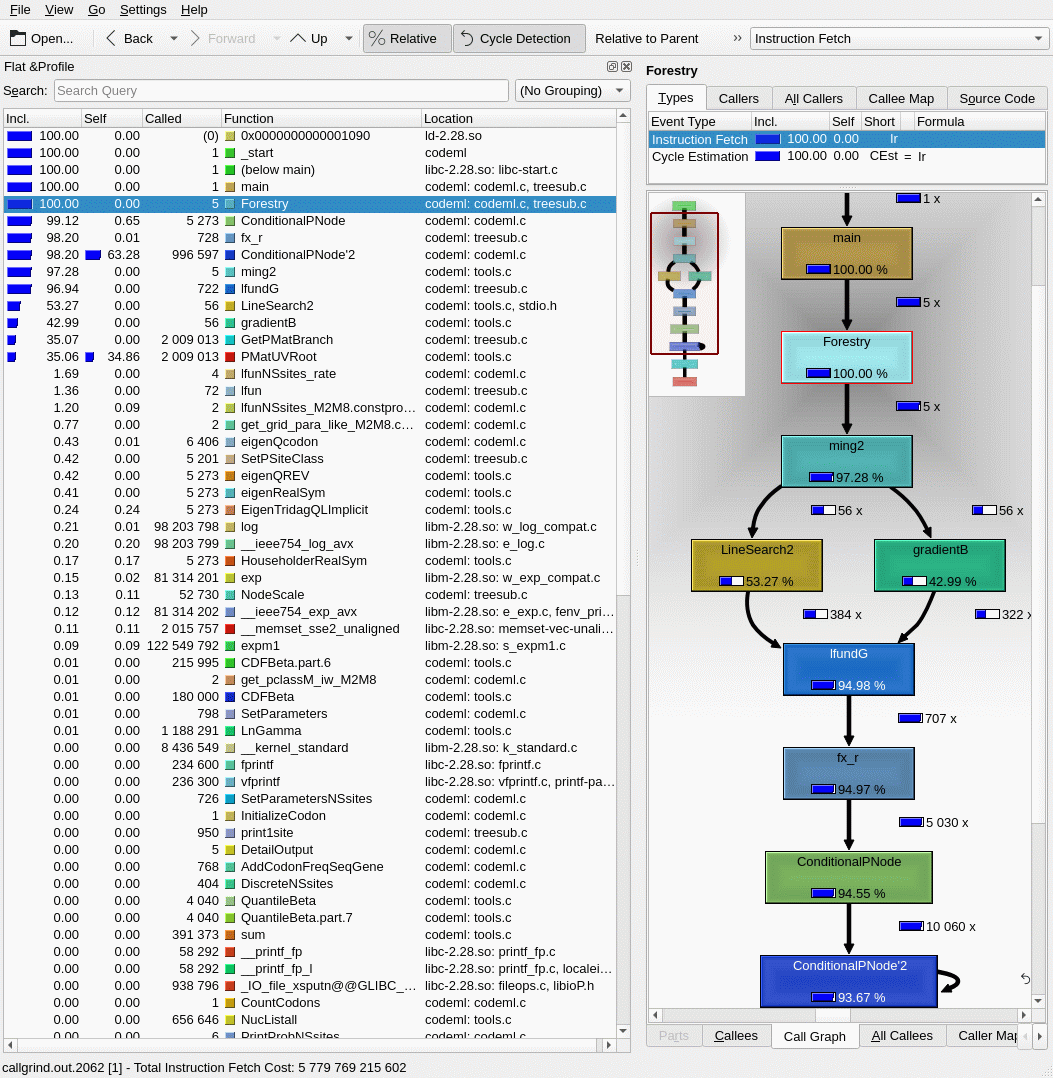
\includegraphics[width=0.3\linewidth]{img/kcachegrind.png} \end{center}
\legend{Fonte: Os Autores} \label{fig:kcachegrind} \end{figure}

Foi considerada uma implementação paralela para todos os métodos numéricos
supracitados. Em um primeiro momento o cálculo do gradiente foi paralelizado
utilizando OpenMP, um modelo de programação paralela para sistemas com
múltiplos processadores com memória compartilhada.\cite{chandra2001parallel} A
escolha de OpenMP se dá por três fatores: ser adequado ao ambiente de trabalho
dos pesquisadores do HCPA (máquinas multiprocessadas), pela simplicidade de uso
para paralelização de laços, e pela disponibilidade nos ambientes utilizados.

O cálculo do gradiente é aproximado utilizando diferenças finitas para obter as
derivadas parciais de primeiro grau. O codeml permite utilizar diferenças
finitas progressivas, centradas, ou regressivas. A paralelização se dá sob
todas variáveis da função cujo gradiente está sendo obtido. O número de threads
foi definido pelo mínimo entre o número de núcleos de processamento disponíveis
e o número de variáveis na função (iterações no laço). Foi utilizado um
escalonador estático com tamanho do bloco igual ao número de variáveis sob o
número de threads, uma vez que a carga de trabalho é homogênea (as variáveis
são todas da mesma função). O algoritmo encontra-se reproduzido abaixo, onde
$p$ é o número de processadores disponíveis, $t$ o número de threads a ser
usado, $c$ o tamanho do bloco, e $n$ o número de variáveis.

\begin{algorithmic}
\State $t \gets \max(1, \min(p, n))$
\State $c \gets \max(1, \frac{n}{t})$
\For{$i \gets 0,n$ \textbf{in parallel}}
  \If{centrada}
    \State $\frac{\partial f}{\partial x_i} \gets \frac{f(x+h)-f(x-h)}{2h}$
  \ElsIf{progressiva}
    \State $\frac{\partial f}{\partial x_i} \gets \frac{f(x+h)-f(x)}{h}$
  \Else
    \State $\frac{\partial f}{\partial x_i} \gets \frac{f(x)-f(x-h)}{h}$
  \EndIf
\EndFor
\end{algorithmic}

A fim de garantir a corretude da implementação paralela foram desenvolvidos
testes unitários para a função. Em um primeiro momento os testes foram
executados tomando como entrada uma função arbitrária com derivada conhecida,
e os resultados da implementação paralela comparados com aqueles obtidos
simplesmente chamando a função derivada \textit{a priori}. Uma vez que esse
teste foi bem sucedido, testou-se como entrada a função sendo derivada na
implementação do codeml.

Os testes revelaram que a implementação paralela gerava resultados diferentes
da sequencial para a função sendo diferenciada no codeml, mas não para funções
arbitrárias com derivada conhecida. O problema consistia da função sendo
diferenciada ter sido implementada de forma não \textit{thread-safe} pelos
autores do codeml, gerando condições de corrida que inviabilizam a simples
paralelização da rotina em questão.

Foi considerado a reimplementação das funções sendo diferenciadas, todavia, o
uso extensivo de variáveis globais e memória compartilhada na implementação
original do codeml demonstrou-se um grande obstáculo para essa abordagem, que
por isso foi abandonada. Foi estudada então a implementação do slimcodeml, que
reorganiza amplas seções do código fonte, na esperança de que tais
dependências pudessem ter sido removidas, possibilitando a implementação
paralela do cálculo do gradiente. Todavia, apesar de melhor organizado, o
slimcodeml ainda apresenta o mesmo compartilhamento de memória e uso de
variáveis globais encontrados na implementação original, inviabilizando essa
estratégia de paralelização nesse software.

A partir daí foram voltadas as atenções para \textit{LineSearch2}, mas não foi
encontrado na literatura implementações paralelas para o método descrito em
\cite{wolfe1978numerical}, e funções auxiliares utilizadas em seu cálculo
apresentavam os mesmos problemas de compartilhamento de memória encontrados nas
outras rotinas estudadas, tanto na implementação original como no slimcodeml,
portanto a paralelização dessa rotina também foi abandonada.

Por fim, as atenções foram voltadas para o próprio \textit{ming2}, cujo método
numérico (BFGS) é iterativo. Foi realizada uma revisão bibliográfica, que
revelou implementações paralelas desse algoritmo para GPU em
\cite{fei2014parallel}. Os resultados mostram que a implementação não
performa bem para entradas pequenas. Foi realizado então um estudo do uso pelo
codeml desse algoritmo, realizando para isso pequenas adaptações no código para
aumentar a verbosidade dos \textit{logs} da aplicação, ao que observoou-se  que
o codeml trabalha com uma entrada fixa de tamanho 61 para esse algoritmo -- o
número códons que traduzem para aminoácidos -- tamanho esse considerado pequeno
com base no estudo supracitado. Dessa forma, conclui-se que uma paralelização
em GPU seria ineficiente. Além disso, a paralelização desse algoritmo é
complexa e de difícil adaptação ao caso do codeml. Dessa forma, essa abordagem
também foi descartada.

Esgotadas todas possibilidades de paralelização das rotinas responsáveis por
quase a totalidade do tempo de execução do codeml para o caso de uso dos
pesquisadores do HCPA, optou-se por fornecer aos pesquisadores as ferramentas
encontradas através de estudo da literatura. Em particular, os pesquisadores
mostraram-se satisfeitos com o uso do slimcodeml como uma alternativa à
implementação original do codeml.

\section{Pacote ANGSD}
\label{sec:angsd}

Outra aplicação utilizada pelo grupo de pesquisa em genética é o pacote ANGSD,
software para análise genética de diferentes populações de uma
espécie.\cite{korneliussen2014angsd} Os pesquisadores utilizam esse software
para determinar se a genética de uma população influencia em alguma
característica específica de seus indivíduos, através de um teste chamado
\textit{Population Branch Statistic} (PBS), caracterizado pela comparação da
frequência de ocorrência de determinados alelos entre pares de
indivíduos de diferentes populações.\cite{yi2010sequencing}

A análise em questão consiste de duas etapas, a primeira utilizando o binário
angsd, a aplicação principal do pacote ANGSD, e a segunda etapa utilizando a
ferramenta realSFS, um utilitário fornecido pelo pacote. A primeira etapa leva
cerca de um dia para cada arquivo de entrada e porventura apresenta uso elevado
de memória, enquanto que a segunda etapa, que recebe como entrada a saída da
etapa anterior, nunca termina a execução devido a uso de memória
proibitivamente elevado, para os dados de entrada dos pesquisadores do HCPA.

A entrada da primeira etapa consiste em arquivos nos formatos BAM ou CRAM,
descritos na seção \ref{sec:formats}, um arquivo de entrada para cada indivíduo
de cada população sob análise. O angsd então utiliza a biblioteca
htslib\cite{bonfield2021htslib} para manipulação desses arquivos.

Uma primeira observação realizada através de reuniões com os pesquisadores é
que esses dados de entrada são obtidos sempre no formato CRAM do projeto 1000
Genomes, e que estava sendo realizada uma etapa de conversão de CRAM para BAM
para uso do angsd. Essa conversão é realizada utilizando o software SAMtools,
descrito em mais detalhes na seção \ref{sec:SAMtools}, e leva algumas horas
para cada arquivo de entrada. Todavia, como observado anteriormente, o angsd
trabalha também com o formato CRAM, fato esse observado através do estudo do
manual da ferramenta. Sendo assim, a etapa de conversão é desnecessária. Essa
observação já economizou algumas horas de execução.

Eliminada essa etapa de pré-processamento dos dados, realizou-se um estudo do
software a fim de elucidar seu funcionamento, para posteriormente realizar um
perfil de seu uso de memória com a ferramenta massif, do software
callgrind.\cite{weidendorfer2008sequential}

Inicialmente realizou-se um estudo do utilitário realSFS, que apresentava o
principal problema de desempenho. Através de um estudo do código fonte foi
observado que o utilitário implementa dois otimizadores, um legado utilizando
BFGS (o mesmo algoritmo usado no pacote PAML) e o padrão utilizando
``Electromagnetism-like Mechanism'', um método estocástico de otimização
não linear que utiliza mecanismos de atração e repulsão para mover
''partículas`` na direção ótima.\cite{5636954} Foi observado ainda que,
independente do otimizador utilizado, a alocação de memória é a mesma. Fatores
que influenciam no uso de memória incluem o número de threads e o número de
sítios considerados. Em ambos os casos há um \textit{trade-off} - ao reduzir o
número de threads o tempo de execução aumenta, e ao reduzir o número de sítios
a confiabilidade dos resultados diminui.\cite{popgen2016angsd} A redução de
ambos é indesejável, visto que o tempo de execução já é muito elevado e a
confiabilidade dos resultados é fundamental.

Foi traçado então um perfil de memória da aplicação utilizando callgrind,
visando elucidar as causas do uso elevado de memória. Esse perfil revelou que a
etapa de otimização supracitada é o principal responsável pelo uso
proibitivamente alto de recursos, e não foram encontradas oportunidades de
melhoria que não afetassem o tempo de execução ou a confiabilidade dos
resultados.

Foi realizada uma reunião com os pesquisadores, em que foi observado que é
possível realizar a mesma análise feita com o angsd (PBS) utilizando o pacote
SAMtools, construído em cima da biblioteca htslib (tal qual o angsd), e que já
era utilizado na etapa de pré-processamento dos dados, seguida de uma análise
estatística dos resultados. Todavia, o pipeline de análise utilizando tais
ferramentas apresentava tempos proibitivamente lentos. Na seção
\ref{sec:SAMtools} é descrito um estudo desse pipeline e o posterior
desenvolvimento de uma ferramenta que otimiza e paraleliza sua execução,
resolvendo o problema de desempenho supracitado. Tal estudo foi realizado em
paralelo ao estudo do angsd descrito acima e, uma vez que os resultados foram
se mostrando mais frutíferos, o foco dese trabalho passou a ser esse
ferramental, a análise pelo angsd sendo substituída pela análise pelo SAMtools
por parte dos pesquisadores.

\section{Pacote SAMtools}
\label{sec:SAMtools}

Conforme mencionado na seção \ref{sec:angsd}, uma aplicação utilizada pelo
grupo de pesquisa em genética é o pacote SAMtools,\cite{li2009sequence}
aplicação amplamente utilizada na literatura para análise de sequências
genéticas.\cite{danecek2021twelve} O samtoools e a ferramenta bcftools que o
acompanha são construídos em cima da biblioteca htslib, dos mesmos autores, que
permite a leitura e manipulação de arquivos de arquivos em formatos diversos
representando sequências genéticas alinhadas, descritos em \ref{sec:formats}.
Dentro outras funcionalidades dessas ferramentas destaca-se a chamada de
variantes, processo de comparação de sequências genéticas
alinhadas.\cite{danecek2021twelve}

Em mais detalhes, a aplicação samtools providencia o comando \textit{view} para
conversão entre formatos de arquivo, filtragem, e extração de porções de um
arquivo, enquanto comandos como \textit{sort} e \textit{merge} permitem
reordenar e agrupar os arquivos de diversas formas, e os comandos
\textit{index} e \textit{faidx} indexam os arquivos para acesso aleatório
rápido. A ferramenta providencia uma série de outras funcionalidades que fogem
ao escopo desse trabalho e estão descritas em \cite{danecek2021twelve}.

Já a aplicação bcftools, parte do pacote SAMtools, providencia comandos para
execução da chamada de variantes -- \textit{mpileup} e \textit{call}, que
calculam as variantes entre as sequências alinhadas lidas e agrupadas através
de um processo descrito em \cite{li2011improving}. O bcftools providencia mais
21 comandos com mais de 230 opções diferentes para diversas análises das
sequências genéticas alinhadas manipuladas pelo samtools. Uma descrição
completa desses comandos foge ao escopo desse trabalho e pode ser encontrada em
\cite{danecek2021twelve}.

Nesse trabalho foi realizado um estudo da literatura por trabalhos realizados a
partir do SAMtools ou que providenciem funcionalidades equivalentes para
chamadas de variantes, além de estudado, otimizado, e paralelizado o pipeline
de análise do grupo de pesquisa do HCPA utilizando o pacote SAMtools para
chamada de variantes, reduzindo o tempo de execução de vários dias para poucas
horas, e desenvolvida uma interface gráfica para execução do pipeline
otimizado.

\subsection{Trabalhos anteriores}
\label{sec:samant}

Em \cite{takeuchi2016cljam} os autores desenvolvem uma aplicação para execução
paralela de chamada de variantes usando a linguagem de programação Clojure. A
aplicação, chamada cljam, não compartilha base de código com o pacote SAMtools,
mas visa implementar o sub-conjunto de suas funcionalidades relevantes à
chamada de variantes. Os autores testam o desempenho de sua implementação
contra o SAMtools em um ambiente multiprocessado, observando que o SAMtools
possui uma performance melhor mesmo rodando com uma única thread, mas defendem
sua aplicação pela simplicidade do código comparada com o SAMtools e
possibilidade de paralelização. Como o tempo de execução é maior que a
implementação original, não foi realizado um estudo mais aprofundado dessa
implementação.

Em \cite{jin2019pvctools} os autores desenvolvem uma ferramenta para execução
paralela de chamada de variantes utilizando a linguagem de programação C++.
Denominada PVCtools, a aplicação implementa um subconjunto de funcionalidades
do SAMtools relevante à chamada de variantes. Os autores testam o desempenho de
sua aplicação em um ambiente multiprocessado, comparando-o com o do SAMtools.
Em particular, os autores utilizam como entrada amostras do genoma humano,
o mesmo caso de uso dos pesquisadores do HCPA. Em mais detalhes, os
autores utilizam uma entrada de 20 amostras de 3,2 GB, totalizando 64 GB,
consideravelmente menor que a utilizada pelos pesquisadores do HCPA. Para essa
entrada a ferramenta é consideravelmente mais rápida que o SAMtools, mas
apresenta um uso de memória consideravelmente mais elevado, de 80 GB. O uso de
memória observado pelos autores seria proibitivamente elevado para o tamanho de
entrada utilizado pelos pesquisadores do HCPA, da mesma forma que ocorre com o
software ANGSD, para o qual procurava-se alternativa justamente devido ao uso
de memória. Devido a esse fator limitante, essa ferramenta também não foi
explorada mais a fundo nesse trabalho.

Em \cite{tarasov2015sambamba} os autores desenvolvem uma aplicação, na
linguagem de programação D, visando ser uma alternativa ao SAMtools para
processamento em paralelo de múltiplas entradas. Os autores relatam tempos de
execução consideravelmente menores que o do SAMtools em ambiente
multiprocessado, para comandos diversos utilizados na chamada de variantes, e
uso de memória semelhante ao do SAMtools. Uma limitação da ferramenta é que, em
suas versões mais recentes, deixou de suportar o formato de entrada CRAM,
justamente aquele fornecido pelo projeto 1000 Genomes e cuja conversão para BAM é
custosa, conforme discutido em \ref{sec:opt}. Mesmo em versões mais antigas,
apenas um dos comandos, de conversão para outros formatos, suporta entradas
CRAM, efetivamente fazendo com que a ferramenta trabalhe apenas com arquivos
BAM. Isso pode ser um fator limitante para o uso prático dessa ferramenta,
visto que o custo da conversão de CRAM para BAM vai além do tempo de execução
da conversão em si, incluindo o custo de armazenamento dos arquivos BAM,
consideravelmente maiores. Além disso, no manual da versão mais atual da
ferramenta consta que a etapa de chamada de variantes ``não é mais
recomendada'', enquanto é mencionado nas notas de lançamento de uma das versões
da aplicação que um comando fundamental à chamada de variantes ``não
foi fortemente testado''.\cite{manual2015sambamba} De qualquer forma, neste
trabalho foram realizados testes de desempenho dessa aplicação, realizando uma
conversão prévia da entrada de CRAM para BAM e considerando o tempo dessa
conversão nos resultados.

Em \cite{herzeel2015elprep} os autores desenvolvem uma aplicação
multiprocessada para preparo dos arquivos de sequência genética alinhadas para
posterior realização do processo de chamada de variantes. A ferramenta,
denominada elPrep, visa substituir o SAMtools e alternativas, realizando o
processamento inteiramente em memória volátil. Os autores observam que isso
incorre em alto uso de RAM quando a chamada de variantes é realizada por
cromossomo, caso de uso dos pesquisadores do HCPA. Para uma amostra (NA12878)
com 15GB, consideravelmente menor que as entradas utilizadas pelos
pesquisadores do HCPA, o software dos autores utilizou 216GB de RAM. No caso de
ambientes com restrição de memória, os autores recomendam o uso de outras
ferramentas para compor o pipeline, incluindo a ferramenta sambamda, descrita
acima, e o próprio SAMtools. Outro fator limitante é que a ferramenta trabalha
apenas com arquivos nos formatos BAM e SAM, sem suporte a CRAM, da mesma forma
que o sambamba. Além disso, não há suporte para alguns dos comandos do
SAMtools utilizados no pipeline de chamada de variantes dos pesquisadores do
HCPA. Vale mencionar que, apesar de implementação própria, os resultados são
idênticos àqueles das ferramentas que o elPrep visa substituir, segundo os
autores. Devido à ausência de suporte a CRAM, uso de RAM proibitivamente
elevado, e ausência de comandos fundamentais à execução do pipeline usado pelos
pesquisadores, não foram realizados testes mais aprofundados dessa ferramenta
nesse trabalho.

Através de um estudo da literatura foram encontradas ferramentas que visam
substituir o SAMtools, melhorando seu tempo de execução através do uso de
técnicas de programação paralela. Todavia, essas ferramentas apresentam
limitações importantes ao caso de uso dos pesquisadores do HCPA. Nomeadamente:
algumas ferramentas possuem tempo de execução superior ao SAMtools apesar do
paralelismo; algumas ferramentas não suportam arquivos no formato CRAM, formato
atualmente usado pelo projeto 1000 Genomes, de onde são obtidos os arquivos de
entrada; algumas ferramentas apresentam uso de memória proibitivamente elevado;
algumas ferramentas possuem implementações próprias sem testes extensivos dos
resultados contra a implementação de referência (SAMtools). Visando superar
essas deficiências estudou-se em detalhe o pipeline de análise realizado pelo
grupo e desenvolveu-se uma ferramenta própria, que ao mesmo tempo reduz o tempo
de processamento utilizando técnicas de processamento paralelo, utiliza a
implementação de referência, apresenta uso de memória controlado, e possui
suporte ao formato CRAM. O desenvolvimento dessa aplicação bem como os
resultados dos testes de desempenho são descritos nas seções seguintes.

\subsection{Fluxo de análise original}

A fim de realizar a chamada de variantes, os pesquisadores primeiro obtém as
sequências genéticas alinhadas de múltiplos indivíduos de pelo menos três
populações no formato CRAM, bem como o genoma de referência no formato FASTA,
descritos na seção \ref{sec:formats}. Todos dados são obtidos do projeto 1000
Genomes.

O fluxo de análise original fornecido pelos pesquisadores pode ser dividido em
três etapas, após a obtenção dos dados. Na primeira etapa é executada uma
conversão de formato de CRAM para BAM utilizando o comando \textit{samtools
view -b}, seguida de uma rotina de indexação dos arquivos utilizando
\textit{samtools index}.

Uma vez convertidos e indexados, cada arquivo de entrada é separado em 22
arquivos de saída, um para cada par de cromossomos autossômicos humanos,
utilizando o comando \textit{samtools view chr}. Essa etapa na sua forma
originalmente usada pelo grupo de pesquisa encontra-se reproduzida na
figura~\ref{fig:stage1_orig}.

\begin{figure}
  \caption{Fluxo de análise original via SAMtools, etapa 1}
    \begin{center}
      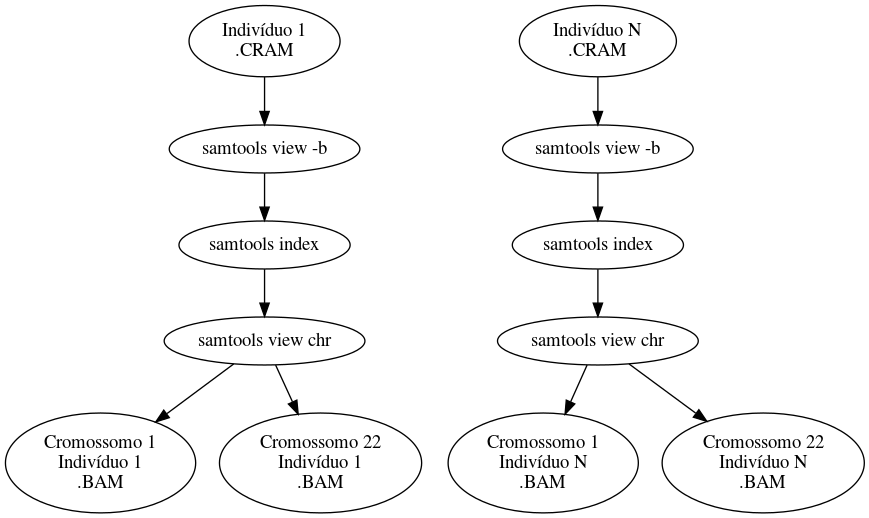
\includegraphics[width=0.85\linewidth]{img/stage1_orig.png}
    \end{center}
    \legend{Fonte: Os Autores}
    \label{fig:stage1_orig}
\end{figure}

Numa segunda etapa, para cada cromossomo são aglutinados os respectivos
arquivos de todos indivíduos, utilizando o comando \textit{samtools merge}.
Posteriormente esses arquivos são indexados, e os comandos \textit{bcftools
mpileup} e \textit{bcftools call} são invocados para executar a chamada de
variantes. O comando \textit{bcftools view} é executado para converter a saída
do formato BCF para VCF, seguido dos comandos \textit{vcftools remove-indels},
que exclui sítios que contenham \textit{indels} (nesse contexto, variantes que
alterem o comprimento do alelo de referência), seguido do comando
\textit{vcftools fiter} para executar um filtro parametrizável por variantes de
interesse. Independente do número de arquivos de entrada, a saída dessa etapa é
sempre 22 arquivos. Ela encontra-se reproduzida na
figura~\ref{fig:stage2_orig}.

\begin{figure}
  \caption{Fluxo de análise original via SAMtools, etapa 2}
    \begin{center}
      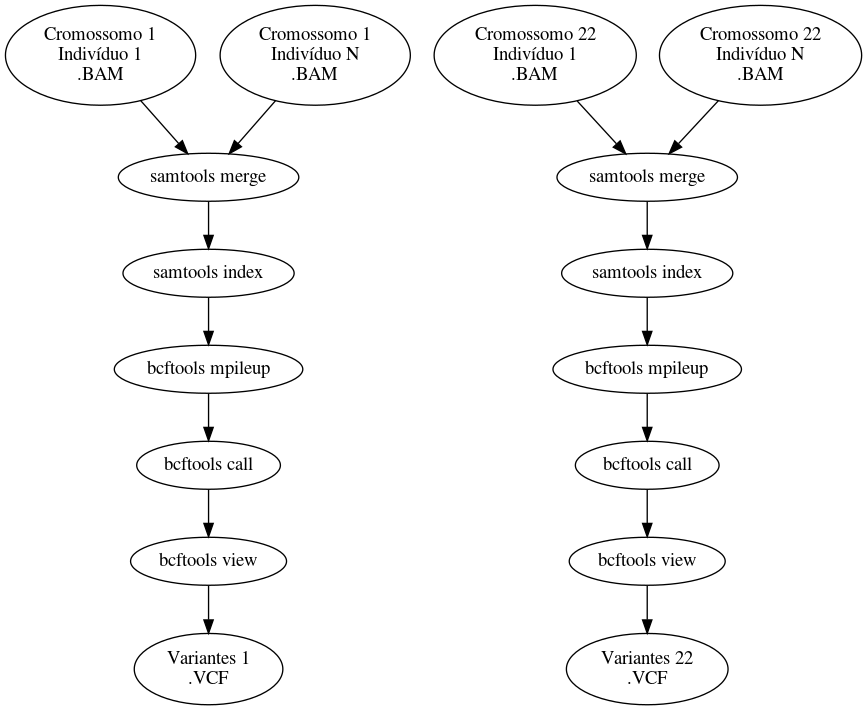
\includegraphics[width=0.85\linewidth]{img/stage2_orig.png}
    \end{center}
    \legend{Fonte: Os Autores}
    \label{fig:stage2_orig}
\end{figure}

A última etapa consiste de concatenar todos arquivos gerados na etapa anterior
utilizando o comando \textit{vcf-concat}, do pacote
VCFtools,\cite{10.1093/bioinformatics/btr330} indexar o arquivo concatenado
utilizando \textit{bcftools index}, e anotar as variantes com a informação
presente no VCF de referência do genoma GRCh38, para isso realizando algumas
conversões de formato via \textit{bcftools view}. Essa etapa recebe sempre 22
arquivos de entrada e produz sempre um único arquivo de saída, e encontra-se
reproduzida na figura \ref{fig:stage3_orig}.

\begin{figure}
  \caption{Fluxo de análise original via SAMtools, etapa 3}
    \begin{center}
      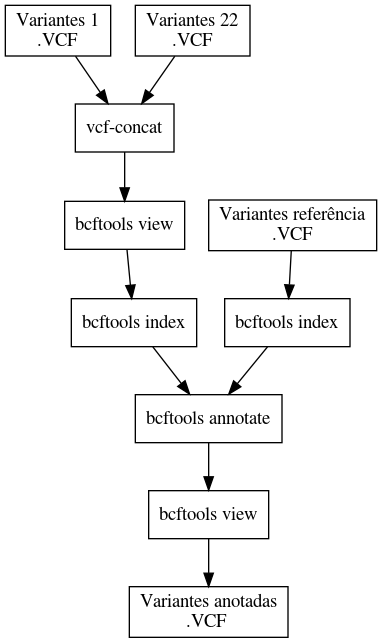
\includegraphics[width=0.85\linewidth]{img/stage3_orig.png}
    \end{center}
    \legend{Fonte: Os Autores}
    \label{fig:stage3_orig}
\end{figure}

Convém ressaltar que os pesquisadores vinham realizando cada uma das etapas
manualmente, porventura repetindo comandos para cada arquivo de entrada ou para
cada cromossomo. Além disso, algumas etapas geram arquivos intermediários que
são necessários somente à etapa posterior, arquivos esses na casa de gigabytes
cada. Isso gerava a necessidade de uma limpeza manual dos arquivos depois de
cada etapa.

\subsection{Fluxo de análise otimizado}
\label{sec:opt}

Através de um estudo da literatura e do manual das ferramentas utilizadas
percebeu-se oportunidade de melhorias no fluxo de análise utilizado pelos
pesquisadores. Em particular, em \cite{danecek2021twelve} os autores observam
que o uso do comando \textit{samtools view -b}, para conversão de CRAM para
BAM, apesar de frequentemente presente em guias na internet é normalmente
desnecessário, uma vez que as ferramentas possuem suporte a CRAM. Isso ocorre
por motivos históricos, pois originalmente o SAMtools não trabalhava com
arquivos CRAM.\cite{danecek2021twelve}

Foram realizados testes de desempenho de cada uma das etapas do fluxo original
de análise, e a conversão de CRAM para BAM era particularmente custosa.
Observado isso, foi testado e comprovado que todo restante da análise poderia
ser executado sem essa etapa, observando o suporte para CRAM e comparando as
saídas do fluxo otimizado com o fluxo original. Dessa forma, essa etapa de
conversão foi removida no fluxo otimizado.

Ainda em \cite{danecek2021twelve} os autores comentam que conversões de BCF
para VCF são custosas e porventura desnecessárias. Na última etapa do fluxo de
análise original é realizada tal conversão seguida de um filtro, para uso dos
arquivos pela ferramenta VCFtools. Apesar do nome, essa ferramenta também
trabalha com arquivos no formato BCF.\cite{man2015vcftools} Foi experimentada a
remoção da etapa de conversão supracitada, substituindo o filtro com o
utilitário \textit{vcfutils} do pacote SAMtools pela filtragem com o próprio
bcftools utilizando o comando \textit{filter}. Com isso foi observado que a
maior parte do tempo de execução está na filtragem e não na conversão, e não
houve diferença significativa de desempenho do VCFtools usando BCF ou VCF. Por
fim, os pesquisadores precisam dos arquivos de saída finais no formato VCF para
análise estatística dos dados em texto plano, portanto uma conversão é
inevitável. Dessa forma, diferente da conversão de CRAM para BAM, a conversão
de BCF para VCF foi mantida no fluxo otimizado.

Na última etapa do fluxo original estava presente uma etapa de indexação das
variantes do genoma de referência, sendo uma etapa custosa, visto que o arquivo
sendo indexado possui 15 GB comprimido, precisa ser descomprimido e depois
indexado. Todavia, o mesmo projeto (NCBI) que fornece o arquivo das variantes
do genoma de referência também fornece o respectivo arquivo de índice, que tem
apenas 2,7 megabytes. Dessa forma, a etapa de indexação foi substituída pelo
download do índice de referência, novamente economizando tempo de execução.

Foi observado ainda que as duas primeiras etapas do fluxo original eram
embaraçosamente paralelas, consistindo de passos independentes para cada
arquivo de entrada.  Como os pesquisadores do HCPA possuem acesso a máquinas
multiprocessadas, foi realizada uma paralelização de ambas etapas utilizado GNU
Parallel\cite{tange_ole_2021_5233953}. A escolha dessa ferramenta se deu pela
facilidade de uso, disponibilidade nos ambientes usados pelos pesquisadores, e
suporte a ajuste automático do número de \textit{jobs} paralelos ao número de
núcleos de processamento disponíveis. Foi desenvolvida uma ferramenta para
execução do fluxo de análise otimizado e paralelizado. Um pseudo código da
ferramenta encontra-se reproduzido abaixo.

\begin{algorithmic}
  \State $C \gets \text{input CRAMs}$
  \State $n \gets \text{input length}$
\For{$j \gets 0,n$ \textbf{in parallel}}
  \State samtools index C(j)
  \For{$i \gets 1,22$}
    \State $R(i,j) \gets \text{samtools view } C(j) \text{ chr i}$
  \EndFor
\EndFor

\For{$i \gets 1,22$ \textbf{in parallel}}
  \State $M(i) \gets \text{samtools merge } R(i,j)$ \textbf{for j in 0,n}
  \State samtools index $M(i)$
  \State bcftools mpileup $M(i)$
  \State bcftools call $M(i)$
  \State bcftools view $M(i)$
  \State vcftools remove-indels $M(i)$
  \State vcftools filter $M(i)$
\EndFor

\State $C \gets \text{vcf-concat } M(i)$ \textbf{for i in 1,22}
\State bcftools view C
\State bcftools index C
\State bcftools annotate C
\State bcftools view C
\end{algorithmic}

As otimizações e a paralelização reduziram drasticamente o tempo total de
execução da análise. Na tabela \ref{tbl:SAMtools} encontram-se reproduzidos os
tempos de execução utilizando o pipeline original e o otimizado. Os testes
foram realizados na máquina Thor1, descrita na tabela \ref{tbl:thor1},
utilizando todos núcleos de processamento disponíveis.

\begin{table}[h]
    \caption{Tempos de execução do SAMtools}
    \centering
        \begin{tabular}{c|c|c}
          \hline
          \textit{Tamanho da entrada}  &   \textit{Tempo original}  & \textit{Tempo otimizado} \\
          \hline
          \hline
          58 GB (2 CRAMs) & 1d 4h 55m & 4h59m \\
          124 GB (4 CRAMs) & 2d 9h 50m & 7h39m \\
          232 GB (8 CRAMs) & 4d 14h 35m & TODO \\
          \hline
        \end{tabular}
      \legend{Fonte: Os autores}
    \label{tbl:SAMtools}
\end{table}

Além disso, foram realizados testes de desempenho para a entrada de 58 GB
utilizando um número diferente de núcleos de processamento, a fim de estimar o
\textit{speedup} bem como a quantidade de tempo economizado pela paralelização,
o resto sendo atribuído às otimizações no fluxo de análise. Os resultados
encontram-se reproduzidos na tabela \ref{tbl:speedup}.

\begin{table}[h]
    \caption{Speedup da ferramenta}
    \centering
        \begin{tabular}{c|c|c}
          \hline
          \textit{Número de núcleos}  &   \textit{Tempo de execução}  & \textit{Speedup} \\
          \hline
          \hline
          1 núcleo & TODO & TODO \\
          2 núcleos & TODO & TODO \\
          4 núcleos & TODO & TODO \\
          6 núcleos & 4h59m & TODO \\
          \hline
        \end{tabular}
      \legend{Fonte: Os autores}
    \label{tbl:speedup}
\end{table}

Observa-se que uma alternativa à paralelizar somente os \textit{jobs} sob cada
entrada seria utilizar um pipeline dos comandos, dado que, para alguns
comandos, a saída de um é a entrada do seguinte. Dessa forma, ambos poderiam
ser executados em paralelo de forma que a saída fosse consumida assim que
gerada. Esse IO poderia ser feito ainda em memória volátil, reduzindo as
escritas e leituras em disco. Um mecanismo para realizar essa tarefa de
comunicação entre processos (IPC) seria pipes POSIX, que fornecem uma interface
simples para direcionar a saída de um programa à entrada do próximo, ambos
rodando em paralelo, usando um buffer em memória volátil para
isso.\cite{immich2003performance} Num ambiente POSIX, pipes são também a
escolha com melhor desempenho para IPC.\cite{immich2003performance}

Todavia, o fato do IO residir em memória volátil incorre em uso mais elevado
desse recurso, justamente o que tentava-se evitar ao buscar uma alternativa a
softwares como ANGSD e PVCtools. Dessa forma, uma vez testado e observado que o
uso de memória tornava-se elevado demais utilizando um pipeline, foi mantida
somente a paralelização de \textit{jobs} sob os arquivos de entrada, com
remoção automática dos arquivos intermediários gerados por cada etapa, operação
antes realizada manualmente pelos pesquisadores. Observa-se que é precisamente
esse tipo de abordagem que tomam os softwares sambamba e elPrep, que apresentam
uso de memória demasiadamente elevado.

Por fim, foram realizados testes de desempenho da ferramenta sambamba, descrita
em \ref{sec:samant}, a fim de comparar com a ferramenta desenvolvida pelos
autores bem como considerar incorporar o uso do sambamba nela. Os resultados
encontram-se descritos na seção \ref{sec:sambamba}.

\subsection{Testes das aplicações sambamba}
\label{sec:sambamba}

Foram realizados testes de desempenho da aplicação sambamba, descrita na seção
\ref{sec:samant}. A conversão de CRAM para BAM para uso da ferramenta foi
realizada usando o samtools, uma vez que o sambamba, apesar de providenciar tal
suporte em suas versões mais antigas, apresentou problemas na leitura dos
arquivos -- no \textit{issue tracker} do projeto há relatos desses problemas, e
a resposta dos autores foi remover o suporte a CRAM completamente. Cada
conversão leva entre duas e três horas para arquivos de entrada entre 22 GB e
34 GB, na máquina Thor1, cujo hardware está descrito na tabela \ref{tbl:thor1}.

Feita a conversão, foram testados individualmente os comandos providenciados
pela ferramenta sambamba, comparando com os comandos equivalentes da ferramenta
samtools. O comando de indexação foi consideravelmente mais lento na ferramenta
sambamba, apesar de usar múltiplos núcleos enquanto o samtools roda
sequencialmente. Enquanto o samtools levou 39s para indexar um CRAM de 26 GB, o
sambamba levou 2m9s para indexar o BAM convertido a partir dele, de 53 GB.

Já para a rotina de visualização de uma região ou cromossomo o sambamba foi
consideravelmente mais rápido. Enquanto o samtools levou 4m5s para visualizar
uma região do arquivo supracitado, o sambamba levou apenas 19s. Já os comandos
de \textit{merge} e \textit{mpileup} não puderam ser executados com o sambamba
-- para o mesmo arquivo em que os comandos mencionados anteriormente rodaram
com sucesso, tais comandos apresentaram erros sobre o formato do arquivo, tanto
na versão mais atual do sambamba como em versões anteriores. A tabela
\ref{tbl:sambamba} sumariza os resultados.

\begin{table}[h]
  \caption{\textit{Benchmark} da ferramenta sambamba}
    \centering
        \begin{tabular}{c|c|c}
          \hline
          \textit{Comando}  &   \textit{Tempo samtools}  & \textit{Tempo sambamba} \\
          \hline
          \hline
          view (convert) & 2h41m & N/A \\
          index & 39s & 2m9s \\
          view region & 4m5s & 19s \\
          merge & 8m & N/A \\
          pileup & 1h3m & N/A \\
          \hline
        \end{tabular}
      \legend{Fonte: Os autores}
    \label{tbl:sambamba}
\end{table}

Observa-se que os resultados não são diretamente comparáveis com aqueles
apresentados em \cite{tarasov2015sambamba}, visto que lá os autores utilizam
arquivos BAM com o SAMtools, enquanto que neste trabalho são utilizados
arquivos CRAM, significativamente menores. Diante desses resultados optou-se
por não incorporar o sambamba à ferramenta desenvolvida. O único cenário em que
seu uso seria benéfico é na visualização das regiões, mas como o sambamba não
trabalha com CRAM seria necessário uma conversão custosa, de várias horas para
cada arquivo de entrada, para uma redução no tempo de execução de poucos
minutos para alguns segundos. No total, não traria benefícios à ferramenta.

\subsection{Ambiente e interface}

Tanto o samtools como o bcftools e a ferramenta desenvolvida pelos autores
requerem um ambiente com uma série de softwares pré-instalados e em versões
específicas, o que porventura gerava dificuldades aos pesquisadores do HCPA.

A fim de superar tais dificuldades, bem como disponibilizar um ambiente para
reprodução fidedigna dos resultados obtidos nesse trabalho, decidiu-se por
utilizar o software Docker, de virtualização a nível de sistema operacional,
que fornece uma série de vantagens para pesquisa
reprodutível.\cite{boettiger2015introduction} A imagem criada está disponível
em repositório público.\cite{dockerme}

Além disso, foi desenvolvida uma interface gráfica para o uso do samtools e
bcftools para chamada de variantes. O intuito é facilitar o uso do ferramental
para profissionais da biologia que porventura não estejam familiarizados com
interfaces por linha de comando.

A interface é executada na máquina local do usuário, que pode configurar uma
máquina remota para execução do pipeline de análise. Além da execução do
pipeline, a interface automatiza uma série de outros passos realizados pelos
pesquisadores, como obtenção dos dados e manipulação dos arquivos de resultado.
A interface permite ainda realizar todas etapas em segundo plano, verificar seu
progresso, e interrompê-las.

Para desenvolvimento da interface optou-se por utilizar a linguagem de
programação Python, amplamente utilizada para computação
científica.\cite{oliphant2007python} A escolha da linguagem se deu
principalmente pelo sua disponibilidade em múltiplos sistemas operacionais,
visto que os usuários (pesquisadores do HCPA) manifestaram interesse em
utilizar a ferramenta nos sistemas operacionais Windows, Linux, e Mac, e há
suporte tanto de interpretadores da linguagem como das bibliotecas utilizadas
para todas essas plataformas.\cite{oliphant2007python} Outro fator que
influenciou a escolha foi a agilidade no desenvolvimento que a linguagem
proporciona.\cite{oliphant2007python}

Foi utilizada a biblioteca \textit{guietta} para criação da interface
gráfica,\cite{guietta} um \textit{wrapper} em cima da biblioteca
\textit{PySide2}, um \textit{binding} para Python da biblioteca multiplataforma
Qt.\cite{loganathan2013pyside} A escolha da biblioteca vem pela sua facilidade
de uso e pela disponibilidade multiplataforma. A figura \ref{fig:samgui}
apresenta uma captura de tela da interface gráfica desenvolvida.

\begin{figure}
  \caption{Captura de tela da interface gráfica ``SAMGUI''}
    \begin{center}
      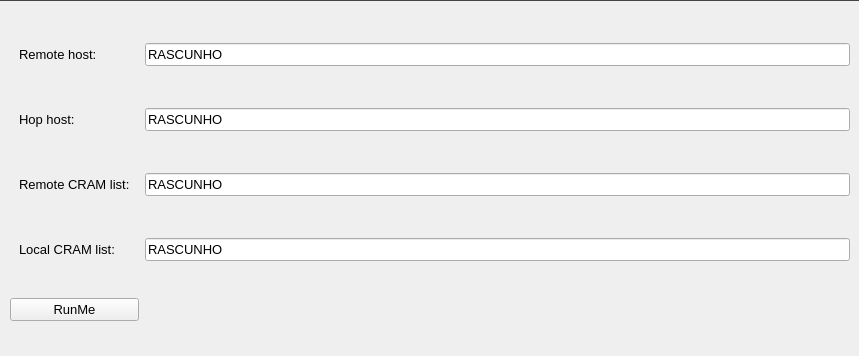
\includegraphics[width=0.85\linewidth]{img/samgui.png}
    \end{center}
    \legend{Fonte: Os Autores}
    \label{fig:samgui}
\end{figure}

\chapter{Conclusão}

Neste trabalho foram estudados os softwares de bioinformática usados pelos
pesquisadores do Hospital de Clínicas de Porto Alegre, nomeadamente os
softwares de análise filogenética e chamada de variantes, com um foco nos
pacotes PAML e SAMtools, que realizam tais tarefas, respectivamente.

No caso dos softwares de análise filogenética foi realizado um estudo da
literatura, análise de desempenho das soluções encontradas e da solução de
referência usada pelos pesquisadores do HCPA (pacote PAML), além de uma
tentativa de paralelização do software original. Com isso, concluiu-se que uma
implementação paralela exigiria grande esforço, provavelmente necessitando uma
reescrita do software para eliminar compartilhamento de memória e uso
abundante de variáveis globais presentes na implementação original que
dificultam sua paralelização. Além disso, foi encontrada solução na literatura
que reduz em mais da metade o tempo de processamento para o caso de uso dos
pesquisadores do HCPA, sendo essa a alternativa adotada para análise
filogenética.

Para os softwares de chamada de variantes também foi realizado uma revisão
bibliográfica e análises de desempenho, além do desenvolvimento de uma
ferramenta própria que paraleliza \textit{jobs} da aplicação de referência
(SAMtools), otimizando o pipeline de chamada de variantes utilizado até então
pelos pesquisadores do HCPA, além de fornecer uma interface gráfica para sua
operação. A escolha de desenvolvimento de uma solução própria que paraleliza
\textit{jobs} da aplicação de referência visa superar deficiências presentes em
soluções encontradas na literatura, nomeadamente o uso elevado de memória, a
ausência de suporte ao formato de arquivo CRAM utilizado pelo projeto 1000
Genomes, e o uso de implementações próprias sem testes extensivos.

Foram realizados testes de desempenho comparando a ferramenta desenvolvida
nesse trabalho com aquelas encontradas na literatura, a ferramenta desenvolvida
pelos autores apresentando uma série de vantagens. Nomeadamente, o uso de
memória foi significativamente inferior àquele das ferramentas ANGSD e
PVCtools, e o uso da implementação da referência (SAMtools) confere maior
confiabilidade à ferramenta versus implementações próprias como no caso da
sambamba, além de suporte a arquivos CRAM. Ao mesmo tempo, a ferramenta
apresenta tempo de execução superior ao uso sequencial da implementação de
referência, e a ausência de necessidade de conversão de CRAM para BAM torna-a
superior em alguns aspectos às ferramentas sambamba e elPrep, sendo uma
alternativa de paralelização de chamada de variantes. Por fim, a
disponibilização de uma interface gráfica facilita o uso por profissionais não
familiarizados com interfaces de linha de comando, e o uso de containers Docker
facilita a reprodução dos resultados obtidos nesse trabalho.

\section{Discussão e trabalho futuro}

Além do pacote SAMtools e softwares alternativos a ele, existem diversas
ferramentas utilizados para chamadas de variante utilizando modelos diferentes
daquele empregado pelo SAMtools. Uma com amplo uso na
literatura\cite{de2017gatk} é a GATK\cite{mckenna2010genome}, que implementa um
modelo de MapReduce para paralelismo das tarefas, inclusive de chamada de
variantes. Outras abordagens ainda mais distantes daquela adotada no SAMtools
envolvem redes neurais, como no caso da ferramenta
DeepVariant,\cite{poplin2018universal} que, apesar de ter tempos de execução
piores que seus pares, possui implementações paralelas recentes que afirmam
superar tais deficiências.\cite{ahmad2021vc} Outra implementação de interesse,
descrita em \cite{massie2013adam}, substitui os formatos de arquivo SAM, BAM,
CRAM, VCF e BCF por uma implementação própria, visando superar algumas de suas
deficiências, além de providenciar APIs para sua manipulação. A implementação é
voltada para frameworks do projeto Apache como Hadoop e Spark, sendo construída
em cima de Apache Parquet e Apache Avro.  Outros trabalhos como
\cite{boufea2017managing} apresentam abordagens semelhantes, enquanto que em
\cite{decap2015halvade} os autores desenvolvem um framework para pipelines de
análise genética incluindo chamada de variantes baseado no GATK utilizando o
modelo de programação MapReduce e o software Apache Hadoop.

Todavia, os métodos empregados e os resultados obtidos na chamada de variantes
utilizando essas e outras ferramentas são diferentes e muitas vezes
complementares àqueles do SAMtools e demais softwares de chamada de
variantes.\cite{gezsi2015variantmetacaller}\cite{guo2015seqmule}

Um trabalho futuro consiste em explorar o uso dessas ferramentas junto aos
pesquisadores do grupo de pesquisa em genética, com avaliação tanto de seu
desempenho como da aplicabilidade desse ferramental considerando os resultados
potencialmente diferentes entre si, para o caso de uso do HCPA, levando em
consideração a literatura a respeito dessas ferramentas.

\bibliographystyle{abntex2-alf}
\bibliography{biblio}

\end{document}
